%! Author = Stepan Oskin
%! Date = 10-Jul-19

% Preamble
\documentclass[11pt]{article}
% Packages
\usepackage{amsmath, subcaption}
\usepackage{graphicx}
\usepackage{amsfonts}

% New commands
\newcommand{\norm}[1]{\left\lVert#1\right\rVert}
\newcommand{\vect}[1]{\boldsymbol{#1}}

% Document
\begin{document}

    \title{Mathematics of the Perceptron learning algorithm\\
    Excerpts from Python Machine Learning \\
    Second Edition \\
    By Sebastian Raschka and Vahid Mirjalili\cite{RaschkaMirjalili2017} \\
    and other sources}

    \author{Stepan Oskin}

    \maketitle

    \begin{abstract}


    \end{abstract}

    \section{Introduction} \label{sec:perc_intro}

    \subsection{Classification} \label{subsec:classification}

    Classifying data is a common task in machine learning.
    Suppose some given data points each belong to one of two classes, and the goal is to decide which class a
    new data point will be in.

    In the case of the perceptron learning algorithm, a data point is viewed as a $p$-dimensional vector
    (a list of $p$ numbers), and we want to know whether we can separate such points with
    a $(p-1)$-dimensional hyperplane.
    This is called a linear classifier.
    More formally, we can put the idea behind artificial neurons into the context of a binary classification task where we refer to our two classes as 1 (positive class) and -1 (negative class) for simplicity.
    There are many hyperplanes that might classify the data.
    We can then define a decision function ($\phi(z)$) that takes a linear combination of certain input values $x$ and a corresponding weight vector $w$, where $z$ is the so-called net input.

    \subsection{McCulloch-Pitts (MCP) neuron} \label{subsec:mcp}

    Trying to understand how the biological brain works, in order to design AI, \textit{Warren McCulloch and Walter Pitts} published the first concept of a simplified brain cell, the so-called McCulloch-Pitts (MCP) neuron, in 1943\cite{McCulloch1990a}.
    Neurons are interconnected nerve cells in the brain that are involved in the processing and transmitting of chemical and electrical signals, which is illustrated in figure~\ref{fig:neuron}:

    \begin{figure}[hbt!]
        \centering
        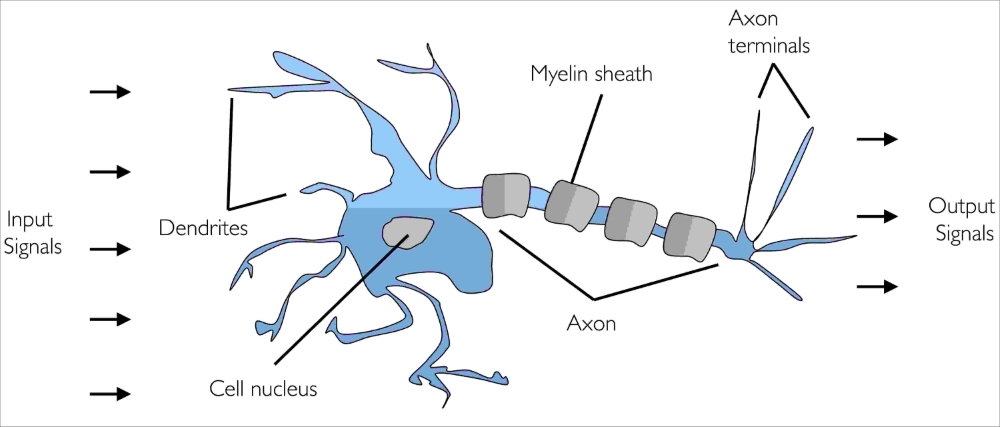
\includegraphics[width=1\linewidth,trim=0.5 0.5 0.5 0.5,clip]{img/neuron.jpg}
        \caption{Neurons are interconnected nerve cells in the brain that are involved in the processing and transmitting of chemical and electrical signals.
        According to the simplified MCP model proposed by McCulloch and Pitts, if the signal accumulated by the dendrites exceeds a certain threshold, an output signal is generated that will be passed on by the axon.}
        \label{fig:neuron}
    \end{figure}

    McCulloch and Pitts described such a nerve cell as a simple logic gate with binary outputs;
    multiple signals arrive at the dendrites, are then integrated into the cell body, and, if the accumulated signal exceeds a certain threshold, an output signal is generated that will be passed on by the axon.

    \subsection{Rosenblatt's Perceptron} \label{subsec:perceptron}

    Only a few years later, \textit{Frank Rosenblatt} published the first concept of the perceptron learning rule based on the MCP neuron model\cite{Rosenblatt1957a}.
    With his perceptron rule, Rosenblatt proposed an algorithm that would automatically learn the optimal weight coefficients that are then multiplied with the input features in order to make the decision of whether a neuron fires or not.
    In the context of supervised learning and classification, such an algorithm could then be used to predict if a sample belongs to one class or the other.

    \section{Mathematics of the perceptron} \label{sec:perc_math}

    \subsection{The formal definition of an artificial neuron} \label{subsec:neuron_def}

    More formally, we can put the idea behind artificial neurons into the context of a binary classification task where we refer to our two classes as 1 (positive class) and -1 (negative class) for simplicity.
    There are many hyperplanes that might classify the data.
    We can then define a decision function ($\phi(z)$) that takes a linear combination of certain input values $x$ and a corresponding weight vector $w$, where $z$ is the so-called net input:

    \begin{equation}
        \label{eq:z}
        \vect{w} = \begin{bmatrix}
                       w_1 \\ \vdots \\ w_m
        \end{bmatrix}, \quad
        \vect{x} = \begin{bmatrix}
                       x_1 \\ \vdots \\ x_m
        \end{bmatrix}, \quad
        z = w_1 x_1 + \dots + w_m x_m
    \end{equation}

    Now, if the net input of a particular sample $\vect{x}^{(i)}$ is greater than a defined threshold $\theta$, we predict class 1, and class -1 otherwise.
    In the perceptron algorithm, the decision function $\phi(.)$ is a variant of a \textbf{unit step function}:

    \begin{equation}
        \label{eq:perc_dec_func}
        \phi(z) =
        \begin{cases}
            1 & {\text{if }}\ z \geq \theta,\\
            -1 & {\text{otherwise}}
        \end{cases}
    \end{equation}

    For simplicity, we can bring the threshold $\theta$ to the left side of the equation and define a weight-zero as $w_0 = - \theta$ and $x_0 = 1$ so that we write $z$ in a more compact form:

    \begin{equation}
        \label{eq:perc_dec_func_bias}
        z = w_0 x_0 + w_1 x_1 + \dots + w_m x_m =
        \sum_{j=0}^m \vect{x}_j \vect{w}_j = \vect{w}^T \vect{x}
    \end{equation}

    In machine learning literature, the negative threshold, or weight, $w_0 = - \theta$, is usually called the \textbf{bias unit}.

    Figure~\ref{fig:perceptron} illustrates how the net input $ z = \vect{w}^T \vect{x} $ is squashed into a binary output (\texttt{-1} or \textt{1}) by the decision function of the perceptron (subfigure~\ref{fig:perc_dec_func}) and how it can be used to discriminate between two linearly separable classes (subfigure~\ref{fig:perc_lin_class}):

    \begin{figure}[hbt!]
        \centering
        \begin{subfigure}[t]{.48\textwidth}
            \centering
            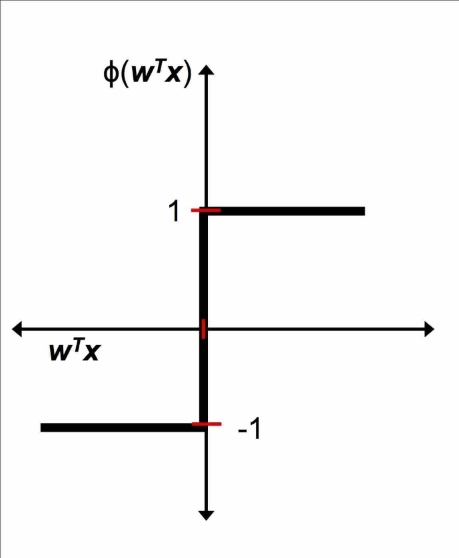
\includegraphics[width=\columnwidth,trim=4 4 4 4,clip]{img/perceptron_a.png}
            \caption{$\gamma=0.2$}
            \label{fig:perc_dec_func}
        \end{subfigure}
        ~ %add desired spacing between images, e. g. ~, \quad, \qquad, \hfill etc.
        %(or a blank line to force the subfigure onto a new line)
        \begin{subfigure}[t]{.48\textwidth}
            \centering
            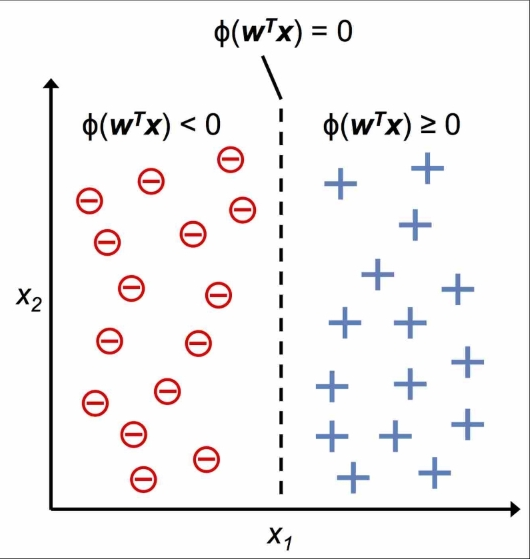
\includegraphics[width=\columnwidth,trim=4 4 4 4,clip]{img/perceptron_b.png}
            \caption{$\gamma=100$}
            \label{fig:perc_lin_class}
        \end{subfigure}
        \caption{.}
        \label{fig:perceptron}
    \end{figure}

    \subsection{The perceptron learning rule} \label{subsec:perc_learn_rule}

    The whole idea behind the MCP neuron and Rosenblatt's \textbf{thresholded} perceptron model is to use a reductionist approach to mimic how a single neuron in the brain works: it either \textbf{fires} or it doesn't.
    Thus, Rosenblatt's initial perceptron rule is fairly simple and can be summarized by the following steps:

    \begin{enumerate}
        \item Initialize the weights to 0 or small random numbers.
        \item For each training sample:
        \begin{enumerate}
            \item Compute the output value.
            \item Update the weights.
        \end{enumerate}
    \end{enumerate}

    Here, the output value is the class label predicted by the unit step function that we defined earlier, and the simultaneous update of each weight $w_j$ in the weight vector $\vect{w}$ can be more formally written as:

    \begin{equation}
        \label{eq:weight_update}
        w_j := w_j + \Delta w_j
    \end{equation}

    The value of $\Delta w_j$, which is used to update the weight $w_j$, is calculated by the perceptron learning rule:

    \begin{equation}
        \label{eq:perc_learn_rule}
        \Delta w_j = \eta \left( y^{(i)} - \hat{y}^{(i)} \right) x_j^{(i)}
    \end{equation}

    Where $\eta$ is the \textbf{learning rate} (typically a constant between 0.0 and 1.0), $y^{(i)}$ is the \textbf{true class label} of the $i^{th}$ training sample, and $\hat{y}^{(i)}$ is the \textbf{predicted class label}.
    It is important to note that all weights in the weight vector are being updated simultaneously, which means that we don't recompute the $\hat{y}^{(i)}$ before all of the weights $\Delta w_j$ are updated.

    A simple diagram presented on figure~\ref{fig:perceptron_dag} illustrates the general concept of the perceptron:
    \begin{figure}[hbt!]
        \centering
        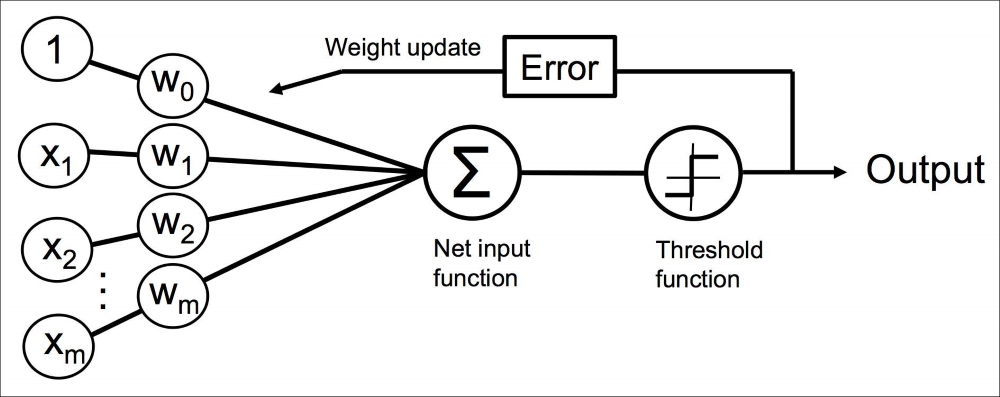
\includegraphics[width=1\linewidth,trim=4 4 4 4,clip]{img/perceptron_dag.jpg}
        \caption{Rosenblatt's thresholded perceptron model uses a reductionist approach to mimic how a single neuron in the brain works: it either fires or it doesn't.
        If the net input of a particular sample $\vect{x}^{(i)}$ is greater than a defined threshold $\theta$, we predict class 1, and class -1 otherwise.}
        \label{fig:perceptron_dag}
    \end{figure}

    The preceding diagram illustrates how the perceptron receives the inputs of a sample $\vect{x}$ and combines them with the weights $\vect{w}$ to compute the net input.
    The net input is then passed on to the threshold function, which generates a binary output \texttt{-1} or \texttt{+1} \textemdash the predicted class label of the sample.
    During the learning phase, this output is used to calculate the error of the prediction and update the weights.

    \subsection{Examples of the perceptron learning rule} \label{subsec:perc_examples}

    Concretely, for a two-dimensional dataset, we would write the weight update using the perceptron learning rule as:

    \begin{equation}
        \label{eq:perc_2var_wupdate}
        \begin{gathered}
            \Delta w_0 = \eta \left( y^{(i)} - \text{output}^{(i)} \right) \\
            \Delta w_1 = \eta \left( y^{(i)} - \text{output}^{(i)} \right) x_1^{(i)} \\
            \Delta w_2 = \eta \left( y^{(i)} - \text{output}^{(i)} \right) x_2^{(i)}
        \end{gathered}
    \end{equation}

    Let us make a simple thought experiment to illustrate how beautifully simple this learning rule really is.
    In the two scenarios where the perceptron predicts the class label correctly, the weights remain unchanged:

    \begin{equation}
        \label{perc_correct}
        \begin{gathered}
            \Delta w_j = \eta \left( -1 - (-1) \right) x_j^{(i)} = 0\\
            \Delta w_j = \eta \left( 1 \textemdash 1 \right) x_j^{(i)} = 0
        \end{gathered}
    \end{equation}

    However, in the case of a wrong prediction, the weights are being pushed towards the direction of the positive or negative target class:

    \begin{equation}
        \label{perc_incorrect}
        \begin{gathered}
            \Delta w_j = \eta \left( 1 - (-1) \right) x_j^{(i)} = \eta \left( 2 \right) x_j^{(i)} \\
            \Delta w_j = \eta \left( -1 - 1) \right) x_j^{(i)} = \eta \left( - 2 \right) x_j^{(i)}
        \end{gathered}
    \end{equation}

    To get a better intuition for the multiplicative factor $x_j^{(i)}$, let us go through another simple example, where:

    \begin{equation}
        \label{eq:perc_example}
        y^{(i)} = +1,~\hat{y}_j^{(i)} = -1,~\eta = 1
    \end{equation}

    Let's assume that $x_j^{(i)} = 0.5$, and we mis-classify this sample as \texttt{-1}.
    In this case, we would increase the corresponding weight by 1 so that the net input $x_j^{(i)} \times w_j^{(i)}$ would be more positive the next time we encounter this sample, and thus be more likely to be above the threshold of the unit step function to classify the sample as \texttt{+1}:

    \begin{equation}
        \label{eq:perc_example_update}
        \Delta w_j^{(i)} = \left( 1 - (-1) \right)0.5 = \left( 2 \right) 0.5 = 1
    \end{equation}

    The weight update is proportional to the value of $x_j^{(i)}$.
    For example, if we have another sample $x_j^{(i)} = 2$ that is incorrectly classified as \texttt{-1}, we'd push the decision boundary by an even larger extent to classify this sample correctly the next time:

    \begin{equation}
        \label{eq:perc_example_update2}
        \Delta w_j^{(i)} = \left( 1 - (-1) \right)2 = \left( 2 \right) 2 = 4
    \end{equation}

    \subsection{Convergence of the perceptron} \label{subsec:perc_conv}

    It is important to note that the \textbf{convergence of the perceptron is only guaranteed} if the two \textbf{classes are linearly separable} and the \textbf{learning rate is sufficiently small}.
    As can be seen in figure~\ref{fig:lin_nonlin}, in some cases the two classes can't be separated by a linear decision boundary.
    In this situation we can set a maximum number of passes over the training dataset (\textbf{epochs}) and/or a threshold for the number of tolerated mis-classifications \textemdash the perceptron would never stop updating the weights otherwise.

    \begin{figure}[hbt!]
        \centering
        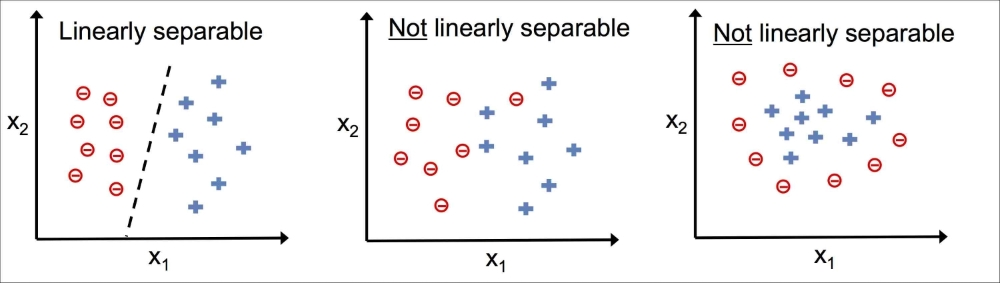
\includegraphics[width=1\linewidth,trim=1 1 1 1,clip]{img/lin_nonlin.jpg}
        \caption{Convergence of the perceptron is only guaranteed if the two classes are linearly separable.
        However, in some cases the two classes can't be separated by a linear decision boundary.}
        \label{fig:lin_nonlin}
    \end{figure}

    \section{An object-oriented perceptron API using NumPy} \label{sec:perc_api}

    For class definition see \texttt{src.classifiers.Perceptron}.
    Code taken from the \textim{book} by {Sebastian Raschka and Vahid Mirjalili}\cite{RaschkaMirjalili2017}.

    \subsection{Description of the implementation} \label{subsec:perc_impl}

    In \texttt{src.classifiers.Perceptron}, an object-oriented approach was taken to define the perceptron interface as a Python class, which allows us to initialize new \texttt{Perceptron} objects that can learn from data via a \texttt{fit} method, and make predictions via a separate \texttt{predict} method.
    As a convention, authors of the code\cite{RaschkaMirjalili2017} append an underscore (\texttt{\_}) to attributes that are not being created upon the initialization of the object but by calling the object's other methods, for example, \texttt{self.w\_}.

    Using this perceptron implementation, new \texttt{Perceptron} objects can now be initialized with a given learning rate \texttt{eta} and \texttt{n\_iter}, which is the number of epochs (passes over the training set).
    Via the \texttt{fit} method, we initialize the weights in \texttt{self.w\_} to a vector $\mathbb{R}^{m+1}$, where $m$ stands for the number of dimensions (features) in the dataset, where we add 1 for the first element in this vector that represents the bias unit.
    Under this convention, the first element in this vector, \texttt{self.w\_[0]}, represents the so-called \textbf{bias unit}.

    \subsection{Initialization of weights} \label{subsec:perc_weights}

    Vector of weights in initialized to small random numbers drawn from a normal distribution with standard deviation \texttt{0.01} via \texttt{rgen.normal(loc=0.0, scale=0.01, size=1 + X.shape[1])}, where \texttt{rgen} is a \texttt{NumPy} random number generator that is seeded with a user-specified random seed so that previous results can be reproduced if desired.

    Now, the reason we don't initialize the weights to zero is that the learning rate $\eta$ (\texttt{eta}) only has an effect on the classification outcome if the weights are initialized to non-zero values.
    If all the weights are initialized to zero, the learning rate parameter \texttt{eta} affects only the scale of the weight vector, not the direction.

    The dot product of two Euclidean vectors $\vect{v1}$ and $\vect{v2}$ is defined as:

    \begin{equation}
        \label{eq:vec_dot}
        \vect{v1} \cdot \vect{v2} = \norm{\vect{v1}} \norm{\vect{v2}} \cos \theta
    \end{equation}

    where $\theta$ is the angle between $v1$ and $v2$.

    We can consider vectors $\vect{v1} = \begin{bmatrix}
                                             1 & 2 & 3
    \end{bmatrix}$ $\vect{v2}=0.5 \times{\vect{v1}}$.
    Using trigonometry, we can show that the angle between $\vect{v1}$ and $\vect{v2}$ would be exactly zero:

    \begin{equation}
        \label{}
        \theta = \arccos{\frac{\vect{v1}\vect{v2}} {\norm{\vect{v1}} \norm{\vect{v2}}}} = 0
    \end{equation}

    \subsection{Fitting the model and making predictions} \label{subsec:perc_fit_predict}

    After the weights have been initialized, the \texttt{fit} method loops over all individual samples in the training set and updates the weights according to the perceptron learning rule that we discussed in the previous section.
    The class labels are predicted by the \texttt{predict} method, which is called in the \texttt{fit} method to predict the class label for the weight update, but \texttt{predict} can also be used to predict the class labels of new data after we have fitted our model.
    Furthermore, we also collect the number of misclassifications during each epoch in the \texttt{self.errors\_} list so that we can later analyze how well our perceptron performed during the training.
    The \texttt{np.dot} function that is used in the \texttt{net\_input} method simply calculates the vector dot product $\vect{w}^T \vect{x}$.

    \subsection{Vectorization} \label{subsec:vectorization}

    Instead of using \textt{NumPy} to calculate the vector dot product between two arrays \texttt{a} and \texttt{b} via \texttt{a.dot(b)} or \texttt{np.dot(a, b)}, we could also perform the calculation in pure Python via \texttt{sum([i * j for i, j in zip(a, b)])}.
    However, the advantage of using \texttt{NumPy} over classic Python for loop structures is that its arithmetic operations are \textbf{vectorized}.
    Vectorization means that an elemental arithmetic operation is automatically applied to all elements in an array.
    By formulating our arithmetic operations as a sequence of instructions on an array, rather than performing a set of operations for each element at the time, we can make better use of our modern CPU architectures with \textbf{Single Instruction, Multiple Data (SIMD)} support.
    Furthermore, \texttt{NumPy} uses highly optimized linear algebra libraries such as \textit{Basic Linear Algebra Subprograms (BLAS)} \textit{and Linear Algebra Package (LAPACK)} that have been written in C or Fortran.
    Lastly, \texttt{NumPy} also allows us to write our code in a more compact and intuitive way using the basics of linear algebra, such as vector and matrix dot products.

    \section{Training a perceptron model on two classes from the Iris dataset} \label{sec:perc_iris}

    To test the perceptron implementation, Iris flower dataset for classification was used, from which two flower classes Setosa and Versicolor were loaded.
    Although the perceptron rule is not restricted to two dimensions, only two features were considered (\texttt{sepal length} and \texttt{petal length}) for visualization purposes.
    Though we only chose the two flower classes Setosa and Versicolor for practical reasons, the perceptron algorithm can be extended to multi-class classification \textemdash for example, the \textbf{One-versus-All (OvA)} technique.

    \subsection{Extracting \texttt{X} and \texttt{y} from Iris dataset} \label{subsec:perc_iris_extract}

    \begin{table}[h!]
        \centering
        \begin{tabular}{||c | c c c c | c||}
            \hline
            index & 0 & 1 & 2 & 3 & 4 \\
            \hline
            \hline
            0 & 5.1 & 3.5 & 1.4 & 0.2 & Iris-setosa \\
            \hline
            1 & 4.9 & 3.0 & 1.4 & 0.2 & Iris-setosa \\
            \hline
            2 & 4.7 & 3.2 & 1.3 & 0.2 & Iris-setosa \\
            \hline
            3 & 4.6 & 3.1 & 1.5 & 0.2 & Iris-setosa \\
            \hline
            4 & 5.0 & 3.6 & 1.4 & 0.2 & Iris-setosa \\
            \hline
        \end{tabular}
        \caption{The first 5 rows from the Iris flower dataset for classification.
        The four features include \texttt{petal\_width}, \texttt{petal\_length}, \texttt{sepal\_width}, and \texttt{sepal\_length}.
        The three class labels are \texttt{Iris-setosa}, \texttt{Iris-versicolor}, and \texttt{Iris-virginica}.}
        \label{tab:iris}

    \end{table}

    Next, we extract the first 100 class labels that correspond to the 50 \texttt{Iris-setosa} and 50 \texttt{Iris-versicolor} flowers, and convert the class labels into the two integer class labels \texttt{1} (\texttt{versicolor}) and \texttt{-1} (\texttt{setosa}) that we assign to a vector \texttt{y}, where the values method of a \texttt{pandas DataFrame} yields the corresponding \texttt{NumPy} representation.

    \begin{figure}[hbt!]
        \centering
        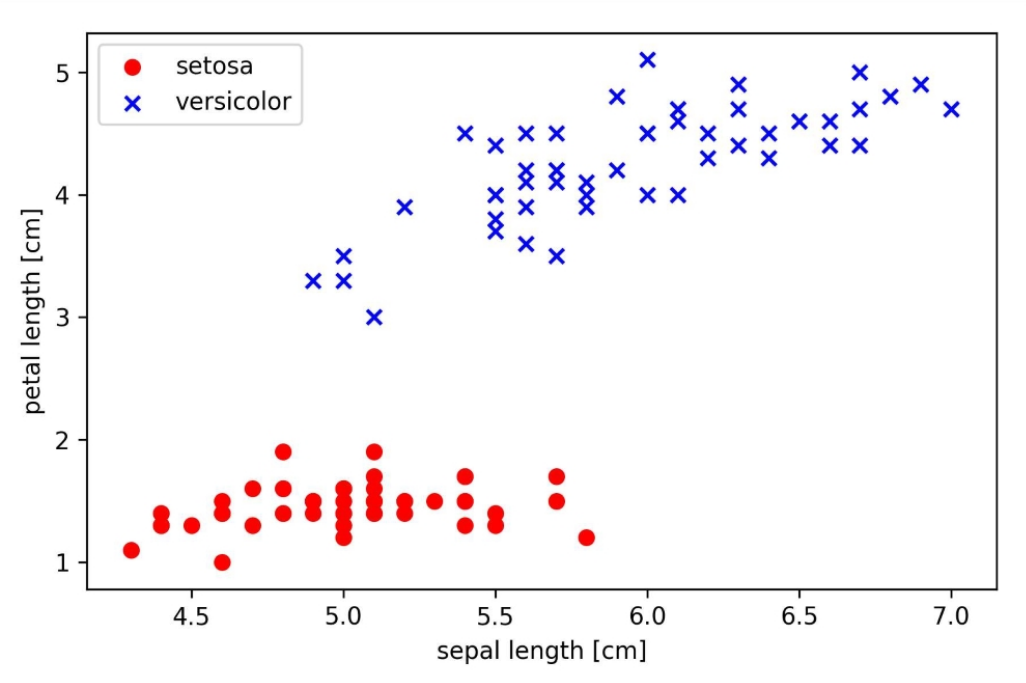
\includegraphics[width=1\linewidth,trim=4 4 4 4,clip]{img/iris_2class.png}
        \caption{We extract the first 100 class labels from Iris dataset that correspond to the 50 \texttt{Iris-setosa} and 50 \texttt{Iris-versicolor} flowers, and convert the class labels into the two integer class labels \texttt{1} (\texttt{versicolor}) and \texttt{-1} (\texttt{setosa}) that we assign to a vector \texttt{y}.
        Similarly, we extract the first feature column (sepal length) and the third feature column (petal length) of those 100 training samples and assign them to a feature matrix \texttt{X}.}
        \label{fig:iris_2class}
    \end{figure}

    Similarly, we extract the first feature column (sepal length) and the third feature column (petal length) of those 100 training samples and assign them to a feature matrix \texttt{X}, which we can visualize via a two-dimensional scatter plot presented in figure~\ref{fig:iris_2class}.
    The scatterplot shows the distribution of flower samples in the Iris dataset along the two feature axes, petal length and sepal length.
    In this two-dimensional feature subspace, we can see that a linear decision boundary should be sufficient to separate Setosa from Versicolor flowers.
    Thus, a linear classifier such as the perceptron should be able to classify the flowers in this dataset perfectly.

    \subsection{Performance of the perceptron on two linearly separable classes} \label{subsec:perc_perf_2class}

    Figure~\ref{fig:perc_updates_epochs} shows the misclassification error for each epoch and can be used to check whether the algorithm converged and found a decision boundary that separates the two Iris flower classes:

    \begin{figure}[hbt!]
        \centering
        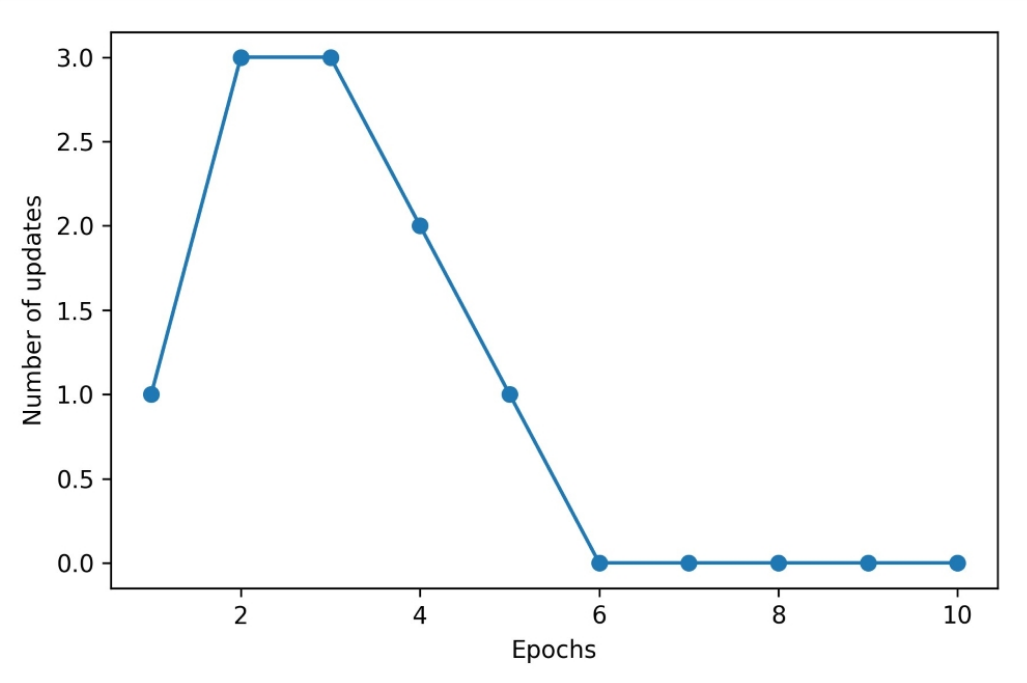
\includegraphics[width=1\linewidth,trim=4 4 4 4,clip]{img/perc_updates_epochs.png}
        \caption{Plotting misclassification error by each epoch shows that the perceptron converged after the sixths epoch and can classify the two classes of Iris flowers perfectly.}
        \label{fig:perc_updates_epochs}
    \end{figure}

    As we can see in the preceding plot, our perceptron converged after the sixth epoch and should be able to classify the training samples perfectly.
    In addition to the number of updates per epoch, decision boundaries can be visualized for two-dimensional datasets.
    Decision boundary learned by the perceptron on the two classes of Iris flowers is presented on figure~\ref{fig:perc_2class_dec_bound}:

    \begin{figure}[hbt!]
        \centering
        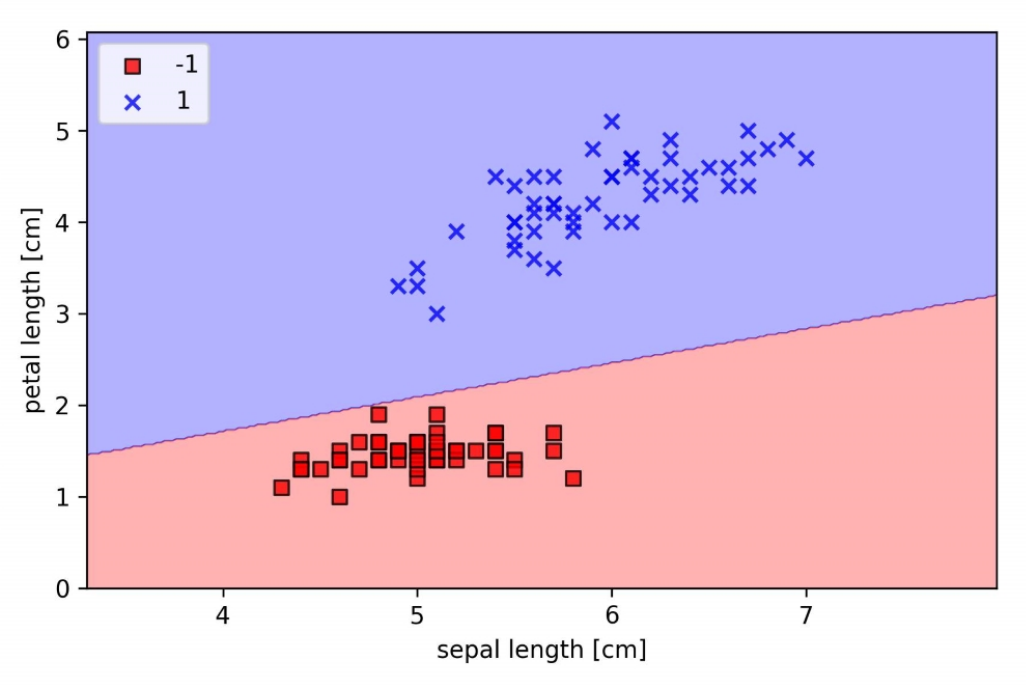
\includegraphics[width=1\linewidth,trim=4 4 4 4,clip]{img/perc_2class_dec_bound.png}
        \caption{Plotting the decision boundary for two features shows that the perceptron learned a decision boundary that is able to classify all flower samples in the Iris training subset perfectly.}
        \label{fig:perc_2class_dec_bound}
    \end{figure}

    As we can see in the plot, the perceptron learned a decision boundary that is able to classify all flower samples in the Iris training subset perfectly.
    Although the perceptron classified the two Iris flower classes perfectly, convergence is one of the biggest problems of the perceptron.
    Frank Rosenblatt proved mathematically that the perceptron learning rule converges if the two classes can be separated by a linear hyperplane.
    However, if classes cannot be separated perfectly by such a linear decision boundary, the weights will never stop updating unless we set a maximum number of epochs.

    \section{Training a perceptron model on three classes from the Iris dataset} \label{sec:perc_preproc}

    \subsection{OvA Technique for multi-class classification} \label{subsec:perc_ova}

    OvA, or sometimes also called \textbf{One-versus-Rest (OvR)}, is a technique that allows us to extend a binary classifier to multi-class problems.
    Using OvA, we can train one classifier per class, where the particular class is treated as the positive class and the samples from all other classes are considered negative classes.
    If we were to classify a new data sample, we would use our n classifiers, where n is the number of class labels, and assign the class label with the highest confidence to the particular sample.
    In the case of the perceptron, we would use OvA to choose the class label that is associated with the largest absolute net input value.

    \subsection{Data preprocessing} \label{subsec:perc_preproc}

    The \texttt{scikit-learn} library offers not only a large variety of learning algorithms, but also many convenient functions to preprocess data and to fine-tune and evaluate our models.
    Conveniently, the Iris dataset is already available via \texttt{scikit-learn}, since it is a simple yet popular dataset that is frequently used for testing and experimenting with algorithms.
    We will only use two features from the Iris dataset for visualization purposes.

    Petal length and petal width of the 150 flower samples was assigned to the feature matrix \texttt{X} and the corresponding class labels of the flower species to the vector \texttt{y}.

    \subsubsection{Encoding target variable} \label{subsec:preproc_encode_target}

    In \texttt{scikit-learn}'s version of the Iris dataset, the Iris flower class names \texttt{Iris-setosa}, \texttt{Iris-versicolor}, and \texttt{Iris-virginica} are already stored as integers (here: `0`, `1`, `2`).
    Although many \texttt{scikit-learn} functions and class methods also work with class labels in string format, using integer labels is a recommended approach to avoid technical glitches and improve computational performance due to a smaller memory footprint;
    furthermore, encoding class labels as integers is a common convention among most machine learning libraries.

    \subsubsection{Train-test split} \label{subsec:preproc_train_test_split}

    To evaluate how well a trained model performs on unseen data, the dataset was split into separate training and test datasets using the \texttt{train\_test\_split} function from \texttt{scikit-learn}'s \texttt{model\_selection} module.
    \texttt{X} and \texttt{y} arrays were randomly split into 30 percent test data (45 samples) and 70 percent training data (105 samples).

    Note that the \texttt{train\_test\_split} function already shuffles the training sets internally before splitting;
    otherwise, all class \texttt{0} and class \texttt{1} samples would have ended up in the training set, and the test set would consist of 45 samples from class 2.
    Via the \texttt{random\_state} parameter, we provided a fixed random seed (\texttt{random\_state=1}) for the internal pseudo-random number generator that is used for shuffling the datasets prior to splitting.
    Using such a fixed \texttt{random\_state} ensures that our results are reproducible.

    Lastly, we took advantage of the built-in support for stratification via \texttt{stratify=y}.
    In this context, stratification means that the \texttt{train\_test\_split} method returns training and test subsets that have the same proportions of class labels as the input dataset.
    NumPy's \texttt{bincount} function, which counts the number of occurrences of each value in an array, can be used to verify that this is indeed the case.

    \subsubsection{Feature scaling} \label{subsec:preproc_feature_scaling}

    Many machine learning and optimization algorithms also require feature scaling for optimal performance.
    Features were standardized using the \texttt{StandardScaler} class from \texttt{scikit-learn}'s \texttt{preprocessing} module:
    Using the \texttt{fit} method, \texttt{StandardScaler} estimated the parameters $\mu$ (sample mean) and $\sigma$ (standard deviation) for each feature dimension from the training data.
    By calling the \texttt{transform} method, we then standardized the training data using those estimated parameters $\mu$ and $\sigma$.
    The same scaling parameters were used to standardize the test set so that both the values in the training and test dataset are comparable to each other.

    \subsection{Training a perceptron on a multi-class dataset using \texttt{scikit-learn}} \label{subsec:perc_sklearn}

    Having standardized the training data, a perceptron model can now be trained on all three classes on Iris flowers.
    Most algorithms in \texttt{scikit-learn} already support multi-class classification by default via the \textbf{One-versus-Rest (OvR)} method, which allows us to feed the three flower classes to the perceptron all at once.
    The \texttt{scikit-learn} interface resembles object-oriented perceptron implementation provided by \textit{Raschka and Mirjalili}\cite{RaschkaMirjalili2017}: after loading the \texttt{Perceptron} class from the \texttt{linear\_model} module, a new \texttt{Perceptron} object is initialized and the model is trained via the \texttt{fit} method.
    Here, the model parameter \texttt{eta0} is equivalent to the learning rate \texttt{eta} that was used in Raschka and Mirjalili's perceptron implementation, and the \texttt{max\_iter} parameter defines the number of epochs (passes over the training set).

    \subsection{Finding an appropriate learning rate} \label{subsec:perc_learn_rate}

    Finding an appropriate learning rate requires some experimentation.
    If the learning rate is too large, the algorithm will overshoot the global cost minimum.
    If the learning rate is too small, the algorithm requires more epochs until convergence, which can make the learning slow \textemdash especially for large datasets.
    \texttt{random\_state} parameter was used to ensure the reproducibility of the initial shuffling of the training dataset after each epoch.

    \subsection{Model accuracy} \label{subsec:perc_accuracy}
    Having trained a model in \texttt{scikit-learn}, predictions can be made via the \texttt{predict} method, just like in Raschka and Mirjalili's perceptron implementation.
    We see that the perceptron misclassifies one out of the 45 flower samples.
    Thus, the misclassification error on the test dataset is approximately 0.0222 or 2.2 percent (1 / 45 = 0.0222).

    Instead of the misclassification error, many machine learning practitioners report the classification accuracy of a model, which is simply calculated as follows:

    Classification accuracy = 1 - error = 0.978 or 97.8 percent.

    \begin{figure}[hbt!]
        \centering
        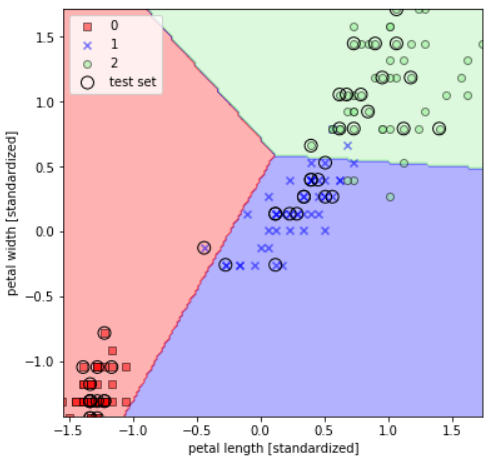
\includegraphics[width=1\linewidth,trim=4 4 4 4,clip]{img/perc_3class_dec_bound.png}
        \caption{For three classes of Iris flowers, the perceptron is able to achieve an accuracy of 98\% on the test set.
        However, since the three classes are not perfectly linearly separable, the perceptron never converges.}
        \label{fig:perc_3class_dec_bound}
    \end{figure}


    \subsection{Decision boundary learned by the perceptron for three classes} \label{subsec:perc_3class_dec_bound}

    For two-dimensional datasets, decision boundary learned by the algorithm can be visualized.
    Decision boundary learned by the perceptron for three classes of Iris flowers is presented on figure~\ref{fig:perc_3class_dec_bound}

    \medskip
    \bibliography{perceptron}
    \bibliographystyle{ieeetr}

\end{document}